\UseRawInputEncoding
\documentclass[12pt]{article}
\title{ECE 102 Homework 2}
\usepackage{subcaption}
\author{Lawrence Liu}
\usepackage{graphicx}
\usepackage{amsmath}
\usepackage[scr]{rsfso}

\newcommand{\Laplace}{\mathscr{L}}
\setlength{\parskip}{\baselineskip}%
\setlength{\parindent}{0pt}%
\usepackage{xcolor}
\usepackage{listings}
\definecolor{backcolour}{rgb}{0.95,0.95,0.92}

\lstdefinestyle{mystyle}{
    backgroundcolor=\color{backcolour}}
\lstset{style=mystyle}

\begin{document}
\maketitle
\section*{Problem 1}
\subsection*{(a)}
After Laplace transform we have that
$$3s^2Y(S)+19sY(s)+20Y(S)=2sX(s)-X(s)$$
$$H(s)=\boxed{\frac{2s-1}{3s^2+19s+20}}$$
\subsection*{(b)}
$$X(s)=\frac{2}{2s+1}e^{-3s}$$
\begin{align*}
Y(s)&=H(s)X(s)\\
&=e^{-3s}\frac{(2s-1)}{(3s^2+19s+20)(s+\frac{1}{2})}\\
&=e^{-3s}\frac{(2s-1)}{(3s+4)(s+5)(s+\frac{1}{2})}\\
&=\frac{e^{-3s}}{3}\frac{(2s-1)}{(s+\frac{4}{3})(s+5)(s+\frac{1}{2})}\\
&=\frac{e^{-3s}}{3}\frac{(2s+1)-2}{(s+\frac{4}{3})(s+5)(s+\frac{1}{2})}\\
&=\frac{e^{-3s}}{3}\left( 2\left(\frac{1}{(s+\frac{4}{3})(s+5)}\right)-\frac{2}{(s+\frac{4}{3})(s+5)(s+\frac{1}{2})}\right)
\end{align*}
We can rewrite 
$$\frac{1}{(s+\frac{4}{3})(s+5)}=\frac{3}{11}\left(\frac{1}{s+\frac{4}{3}}-\frac{1}{s+5}\right)$$
and 
$$\frac{1}{(s+\frac{4}{3})(s+5)(s+\frac{1}{2})}=-\frac{18}{55}\frac{1}{s+\frac{4}{3}}+\frac{2}{33}\frac{1}{s+5}+\frac{4}{15}\frac{1}{s+\frac{1}{2}}$$

Thus we have that
$$y(t)=\boxed{\frac{2}{3}\left(\frac{-3}{55}e^{-\frac{4}{3}(t-3)}+\frac{-11}{33}e^{-5(t-3)}-\frac{4}{15}e^{-\frac{1}{2}(t-3)}\right)u(t-3)}$$

\section*{Problem 2}
\subsection*{(a)}
The system response function is
$$h(s)=\frac{2s^2-14s-16}{s^2+6s^2+11s+6}$$
$$h(s)=\frac{2}{s+2}\frac{1}{s+3}(s-8)$$
Thus the system looks like
\begin{center}
\begin{figure}[h]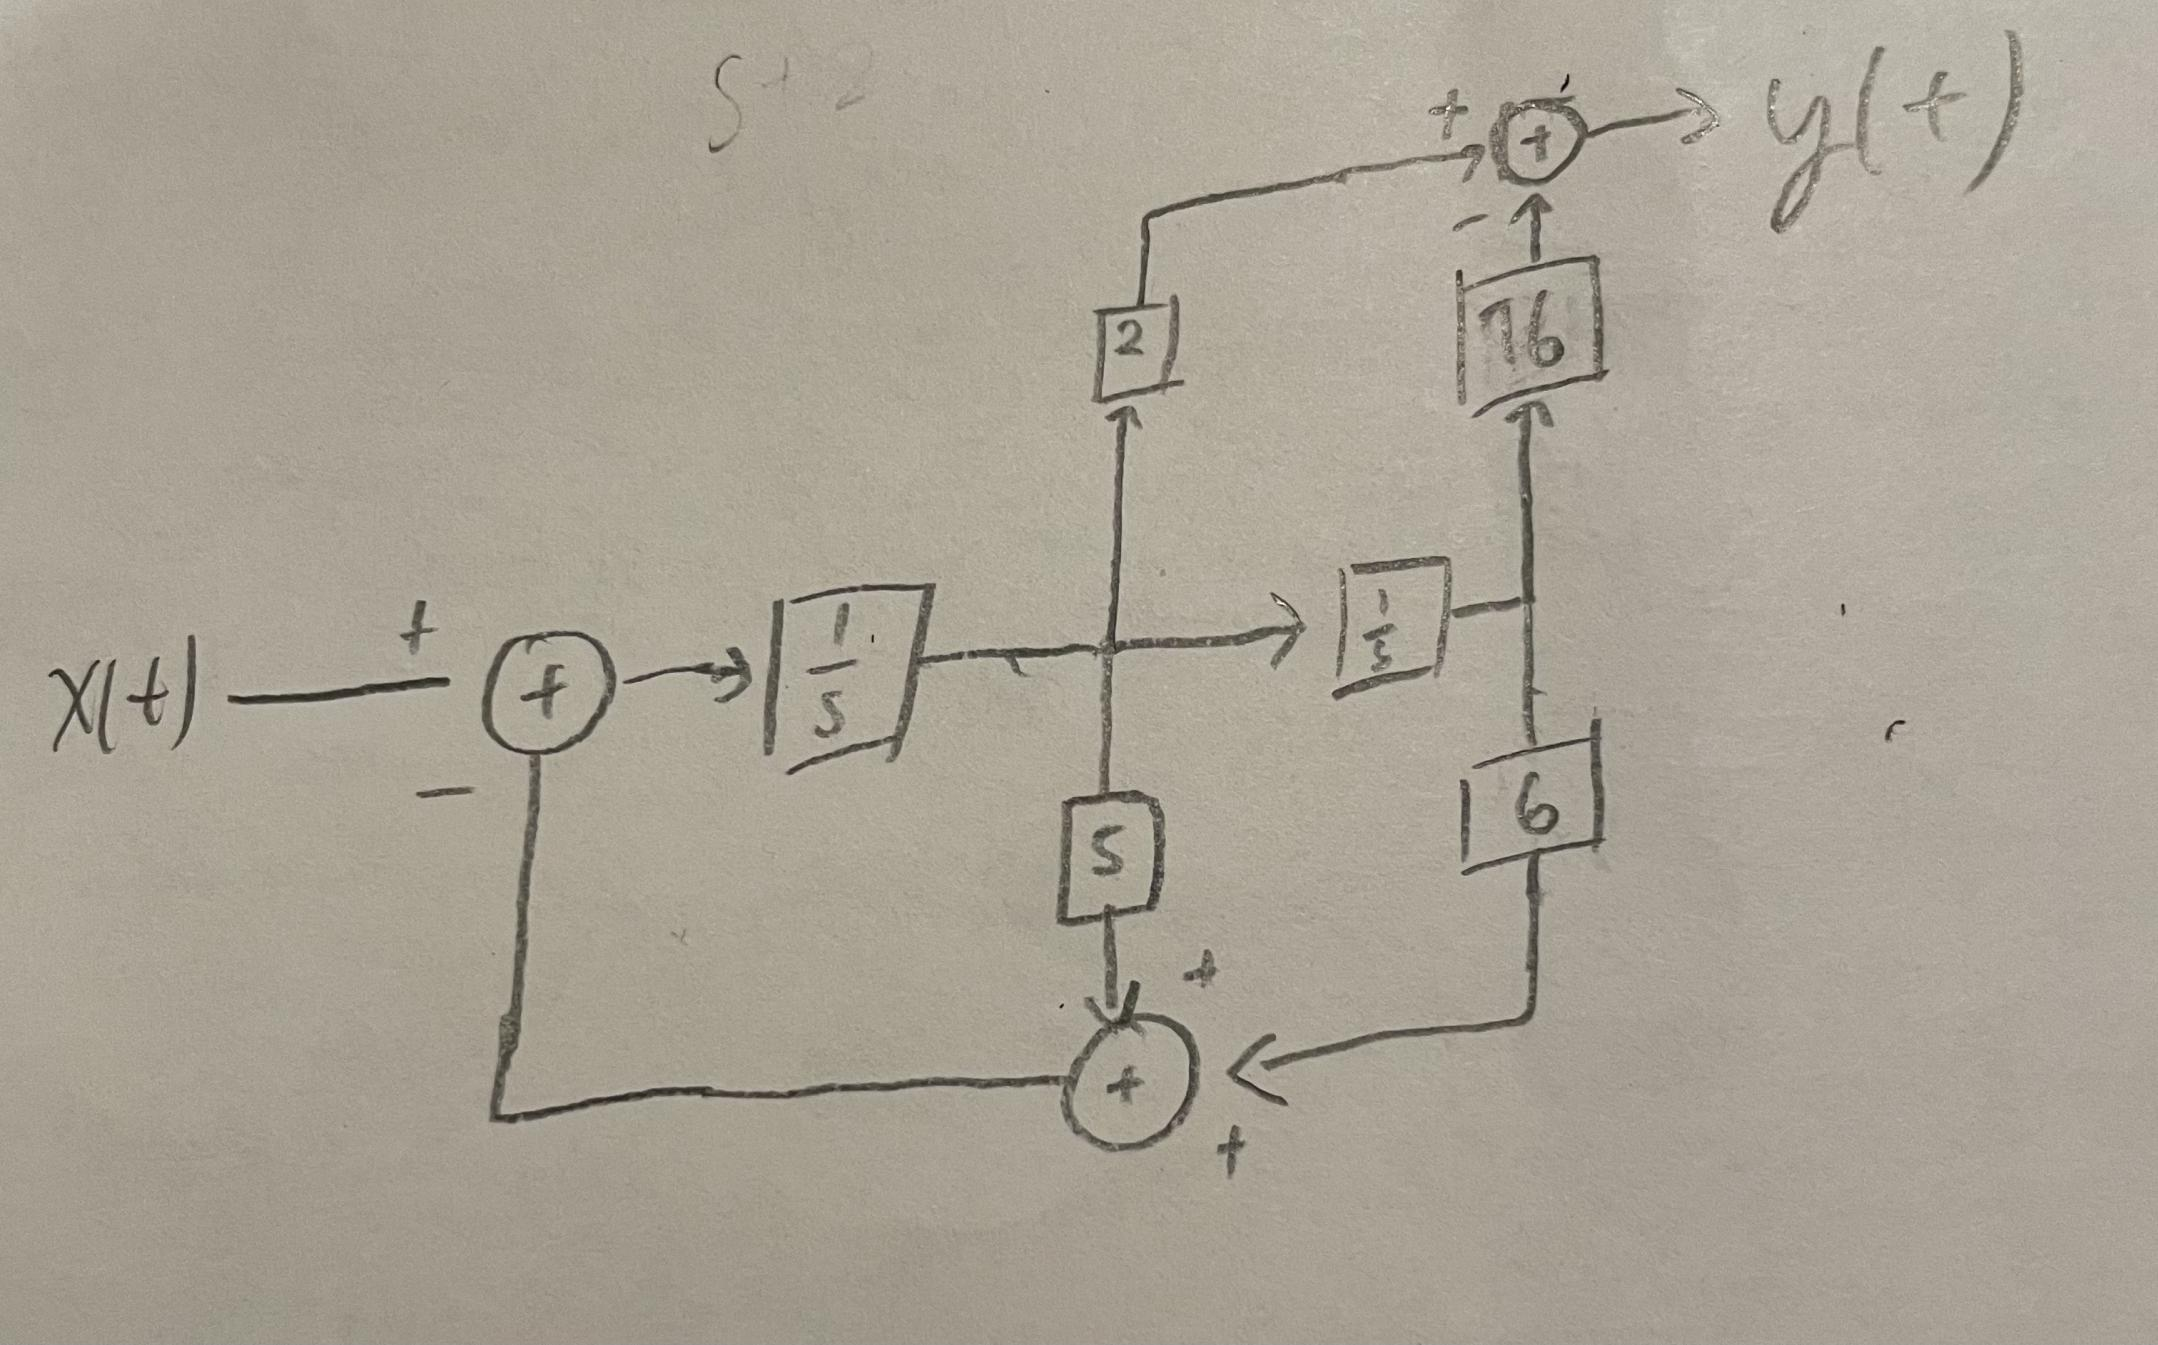
\includegraphics[width=10cm]{fig1}
\end{figure}
\end{center}
\subsection*{(b)}
\begin{center}
\begin{figure}[h]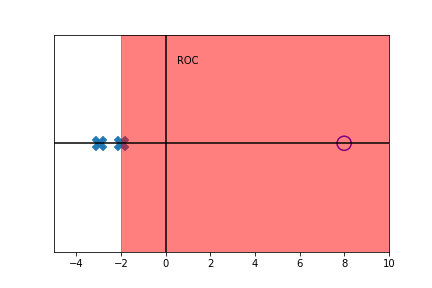
\includegraphics[width=10cm]{fig2}
\end{figure}
\end{center}
This converges since the roc includes $s=0$
\subsection*{(c)}
$$X(s)=\frac{1}{s}\left(e^{2s}-e^{-2s}\right)$$
\begin{align*}
Y(s)&=X(s)H(s)\\
&=\left(e^{2s}-e^{-2s}\right)\frac{2(s-8)}{s(s+2)(s+3)}\\
&=-2\left(e^{2s}-e^{-2s}\right)\left(\frac{1}{(s+2)(s+3)}-8\frac{1}{s(s+2)(s+3)}\right)
\end{align*}
Expanding

$$\frac{1}{(s+2)(s+3)}=\frac{1}{s+2}-\frac{1}{s+3}$$
$$\frac{1}{s(s+2)(s+3)}=\frac{1}{6s}-\frac{1}{2(s+2)}+\frac{1}{3(s+3)}$$

Thus we get that
$$\frac{1}{(s+2)(s+3)}-8\frac{1}{s(s+2)(s+3)}=\frac{5}{s+2}-\frac{4}{3s}-\frac{11}{3(s+3)}$$


Reverse Laplace transforming we get that

$$y(t)=\boxed{2\left(-\frac{4}{3}+5e^{-2(t-2)}-\frac{11}{3}e^{-3(t-2)}\right)u(t-2)-2\left(-\frac{4}{3}+5e^{-2(t+2)}-\frac{11}{3}e^{-3(t+2)}\right)u(t+2)}$$
\section*{Problem 3}
\subsection*{(a)}
Let $a(t)$, $b(t)$, and $c(t)$ be determined as depicted in the drawing below
\begin{center}
\begin{figure}[h]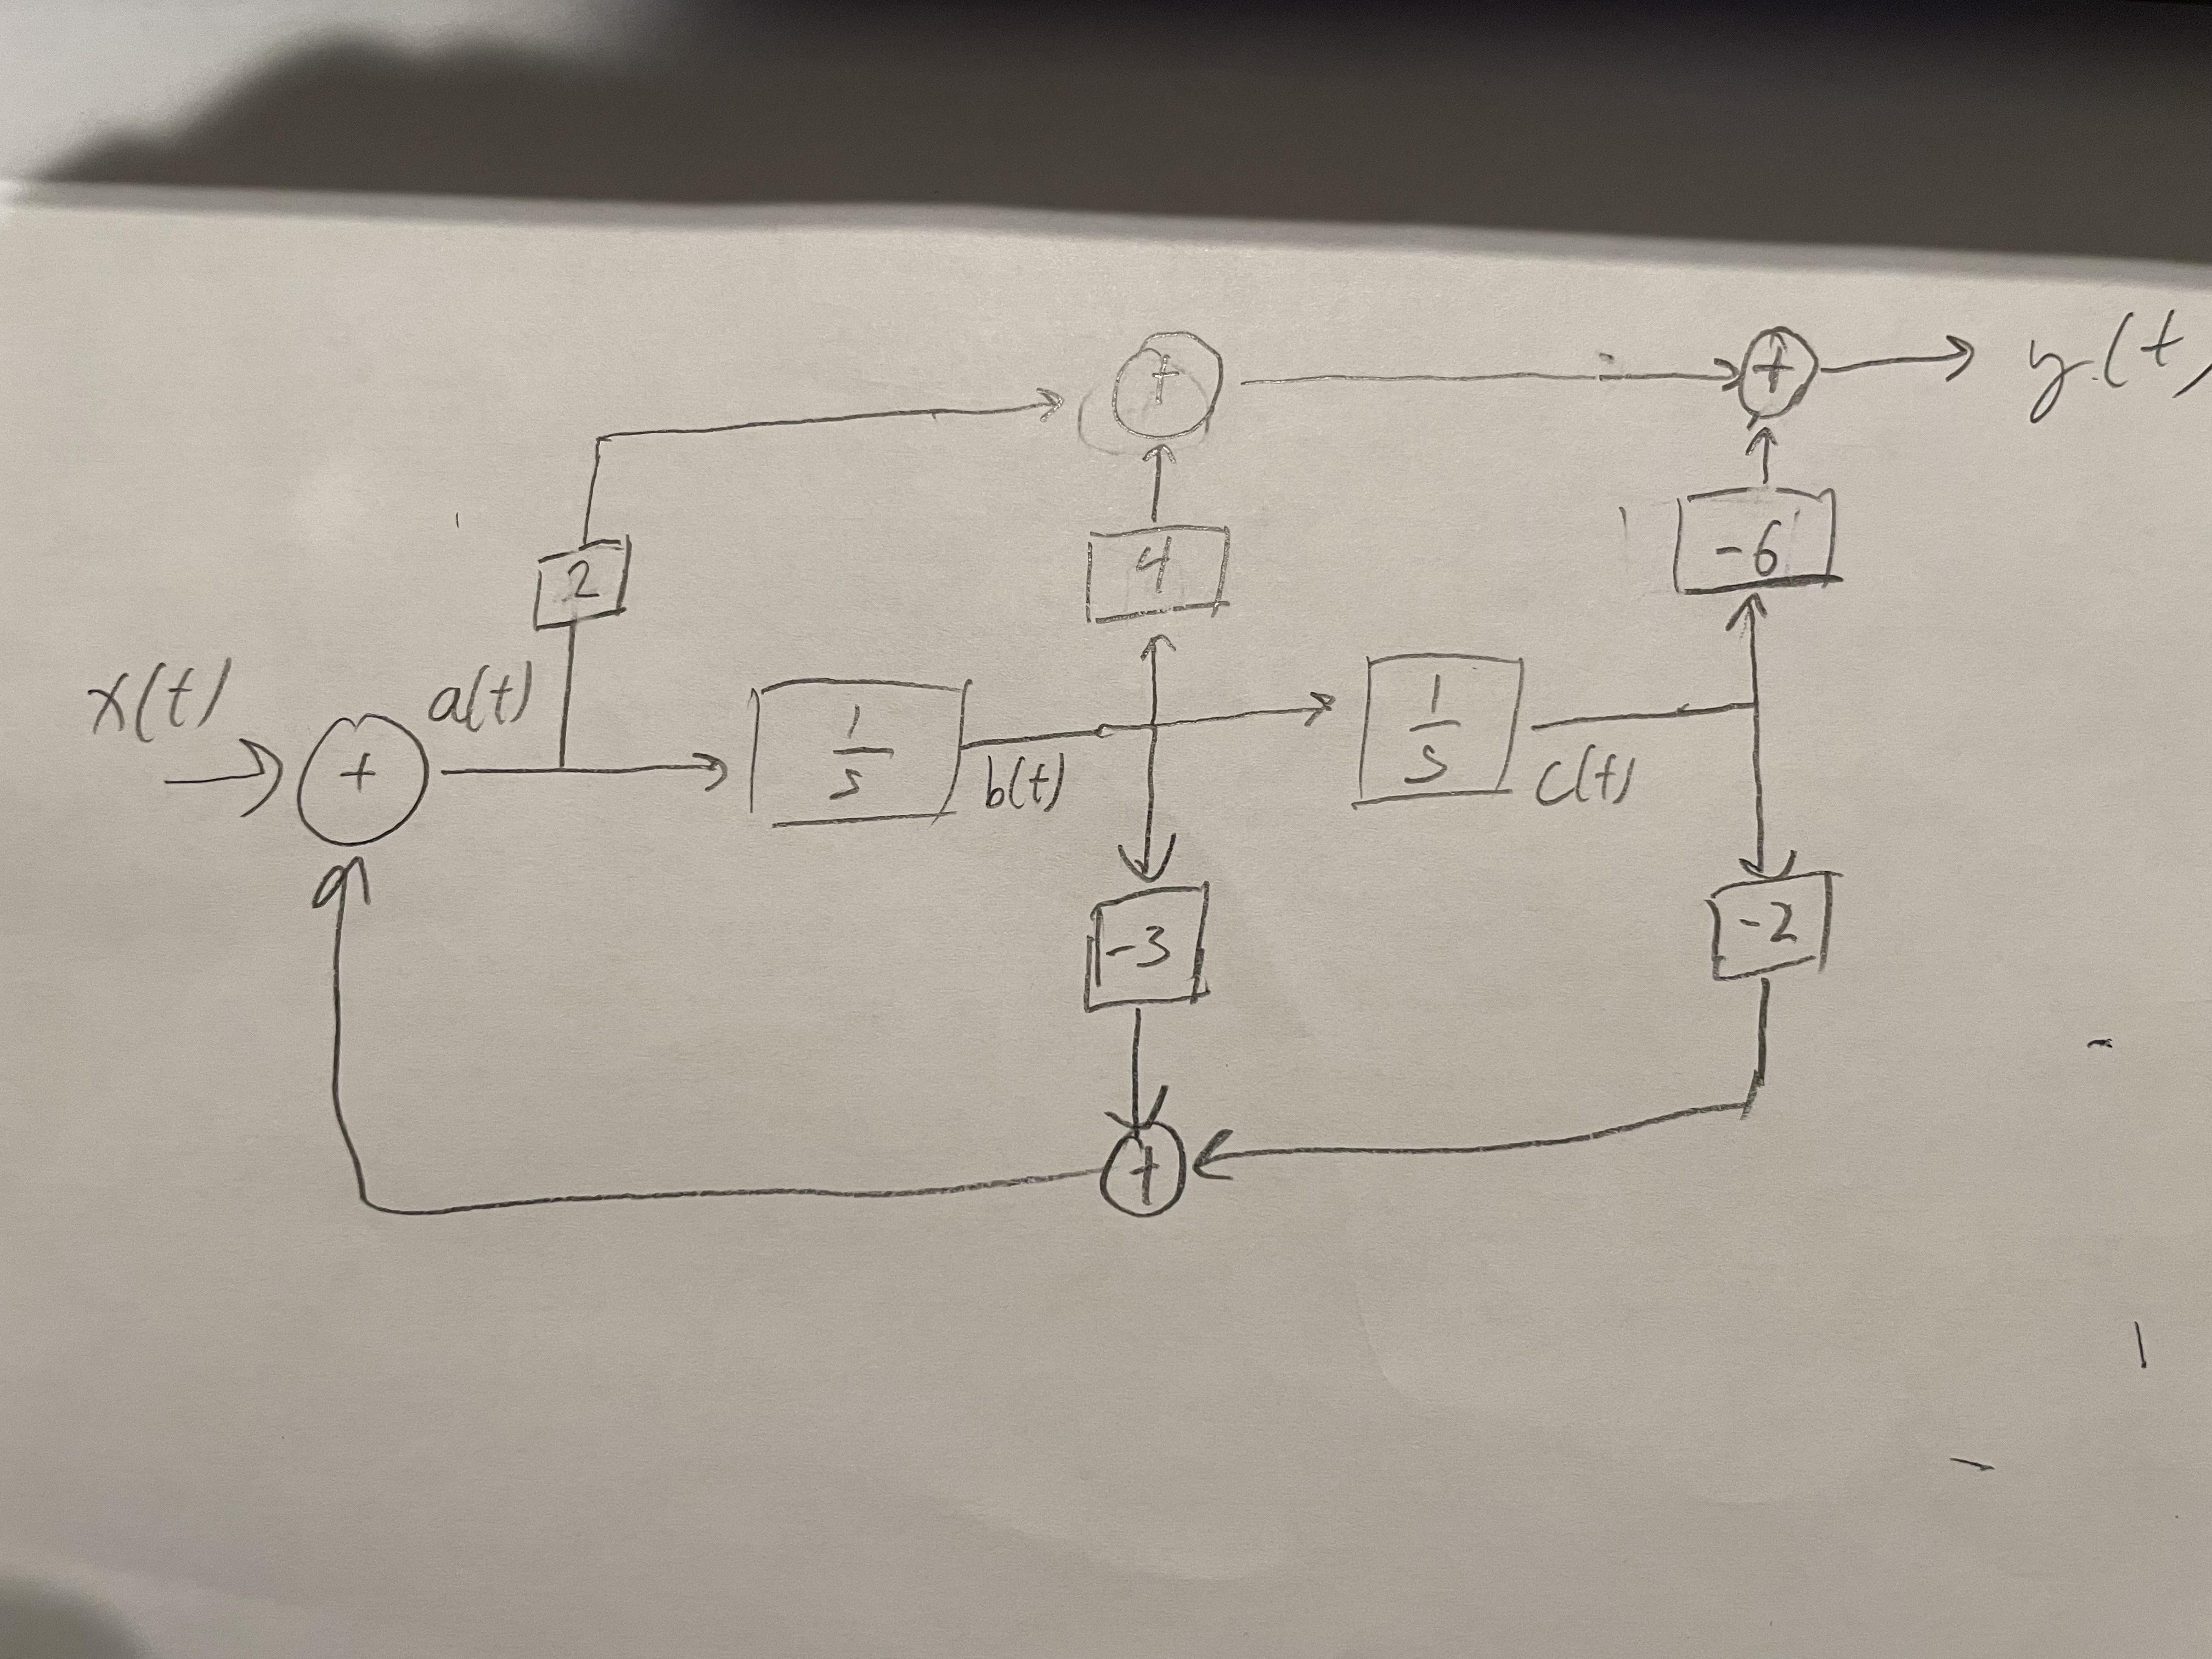
\includegraphics[width=10cm]{fig3}
\end{figure}
\end{center}

Therefore in the $s$ domain we have
$$A(s)=X(s)-3B(s)-2C(s)$$
$$B(s)=\frac{1}{s}A(s)$$
$$C(s)=\frac{1}{s}B(s)=\frac{1}{s^2}A(s)$$


Therefore we have that 
$$A(s)=X(s)-\frac{3}{s}A(s)-\frac{2}{s^2}A(s)$$
$$A(s)=X(s)\frac{1}{1+\frac{3}{s}+\frac{2}{s^2}}$$
$$A(s)=X(s)\frac{s^2}{s^2+3s+2}$$
Thus we have that 
\begin{align*}
Y(s)&=2A(s)+4B(s)-6C(s)\\
&=X(s)\frac{s^2}{s^2+3s+2}\left(2+4\frac{1}{s}-6\frac{1}{s^2}\right)\\
&=X(s)\frac{s^2}{s^2+3s+2}\frac{2s^2+4s-6}{s^2}\\
&=X(s)\frac{2s^2+4s-6}{s^2+3s+2}
\end{align*}

Thus we have that
$$H(s)=\boxed{\frac{2s^2+4s-6}{s^2+3s+2}}$$
\subsection*{(b)}
We have that
$$H(s)=\frac{Y(s)}{X(s)}=\frac{2s^2+4s-6}{s^2+3s+2}$$
$$Y(s)(s^2+3s+2)=X(s)(2s^2+4s-6)$$
Inverse laplace transforming we get that
$$\boxed{\frac{d^2y(t)}{dt^2}+3\frac{dy(t)}{dt}+2y(t)=2\frac{d^2x(t)}{dt^2}+4\frac{dx(t)}{dt}-6x(t)}$$
\subsection*{(c)}
\begin{align*}
H(s)&=\frac{2s^2+4s-6}{s^2+3s+2}\\
&=\frac{2s^2+4s-6}{(s+1)(s+2)}\\
&=\frac{2s}{s+1}-\frac{6}{(s+1)(s+2)}\\
&=\frac{2s+2-2}{s+1}-\frac{6}{s+1}+\frac{6}{s+2}\\
&=2-\frac{8}{s+1}+\frac{6}{s+2}
\end{align*}

Inverse laplace transforming we get that
$$h(t)=2\delta(t)-8e^{-t}+6e^{-2t}$$

\begin{align*}
H(\frac{s}{3})&\to \frac{1}{3}h(3t)\\
H(\frac{s}{3}-4)&\to\frac{1}{3}e^{4t}h(3t)\\
e^{-4s}H(\frac{s}{3}-4)&\to\frac{1}{3}e^{4(t-4)}h(3(t-4))\\
e^{-4s}H(\frac{s}{3}-4)&\to\boxed{\frac{1}{3}e^{4(t-4)}\left(2\delta(3(t-4))-8e^{-3(t-4)}+6e^{-6(t-4)}\right)}
\end{align*}
\section*{Problem 4}
\subsection*{(a)}
$$\Omega_k=\boxed{\frac{2k\pi}{T_0}}$$
\subsection*{(b)}
The period of $\cos(2\pi t)$ is $1$ and the period of $\cos(6\pi t +\frac{\pi}{4})$ is $\frac{1}{3}$, the period of $x(t)$ is the least common multiple of these two, so the period of $x(t)$ is $1$.

Therefore we also have that 
$$A_0=2$$
$$\Omega_0=0$$
$$\theta_0=0$$
$$A_1=1$$
$$\Omega_1=2\pi$$
$$\theta_1=0$$
$$A_3=-3$$
$$\Omega_3=6\pi$$
$$\theta_3=\frac{\pi}{4}$$
\subsection*{(c)}
The period of $\cos(2\pi t)$ is $1$ and the period of $\cos(20t+\frac{3}{4})$ is $\frac{\pi}{10}$. There is no least common multiple of these two. So the signal is not periodic. Since in order for a signal to have a fourier series, it must be periodic, a fourier series cannot be determined for $x_1(t)$
\section*{Problem 5}
\subsection*{(a)}
\lstinputlisting[language=Matlab]{Problem5a.m}
Thus we get

$$F(s)=\boxed{\frac{150}{(s + 3)^4} - \frac{2500}{(s + 3)^3} - \frac{600}{(s + 3)^5} + \frac{120}{(s + 3)^6} - \frac{3125(s + 2)}{(s + 3)^2}} $$ 
\subsection*{(b)}
\lstinputlisting[language=Matlab]{Problem5b.m}

Thus we get
$$f(t)=0.1962 - 0.1962e^{-2.0t}(\cos(1.047t) + 1.91\sin(1.047t))$$

The plot of which looks like
\begin{center}
\begin{figure}[h]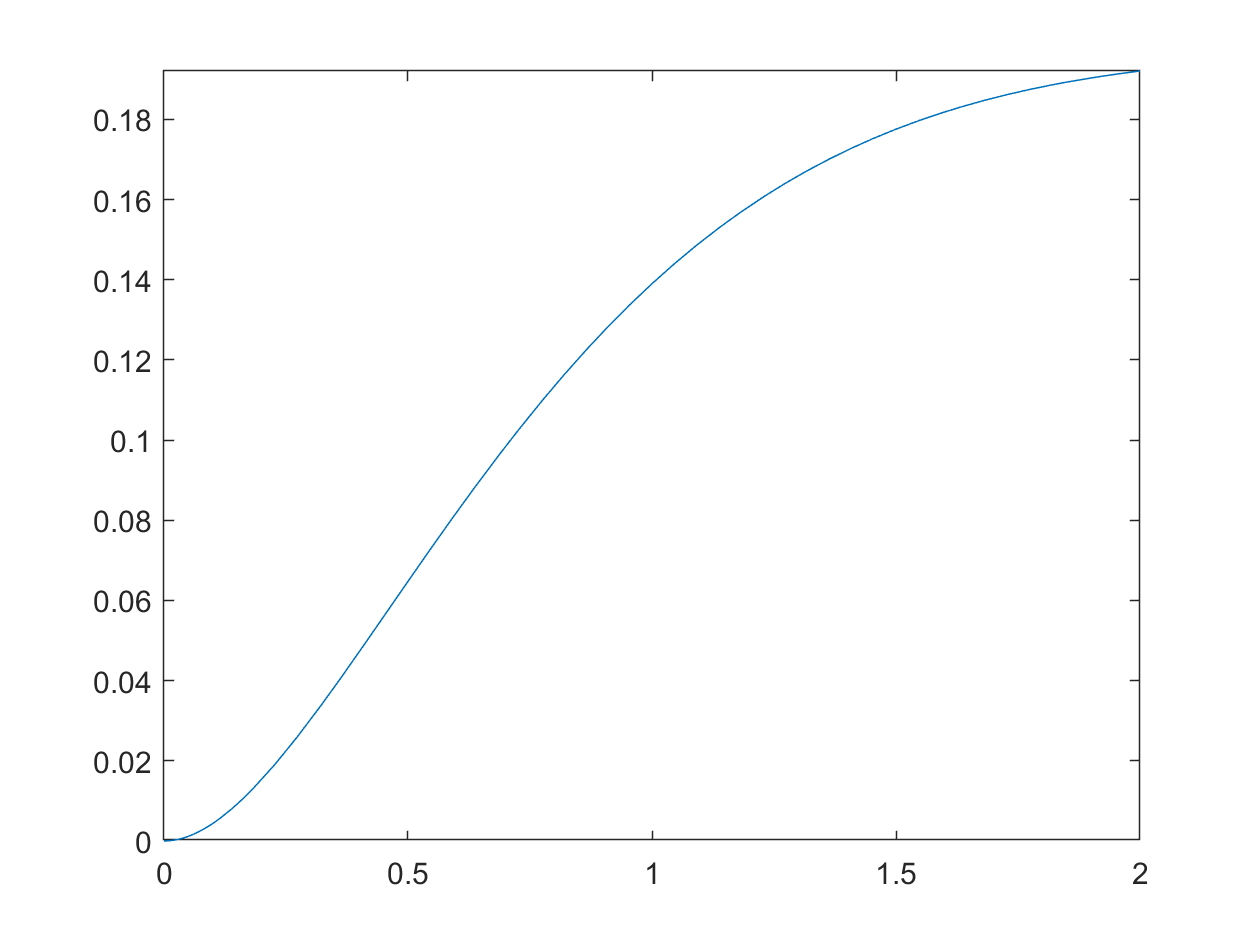
\includegraphics[width=8cm]{fig4}
\end{figure}
\end{center}
\end{document}